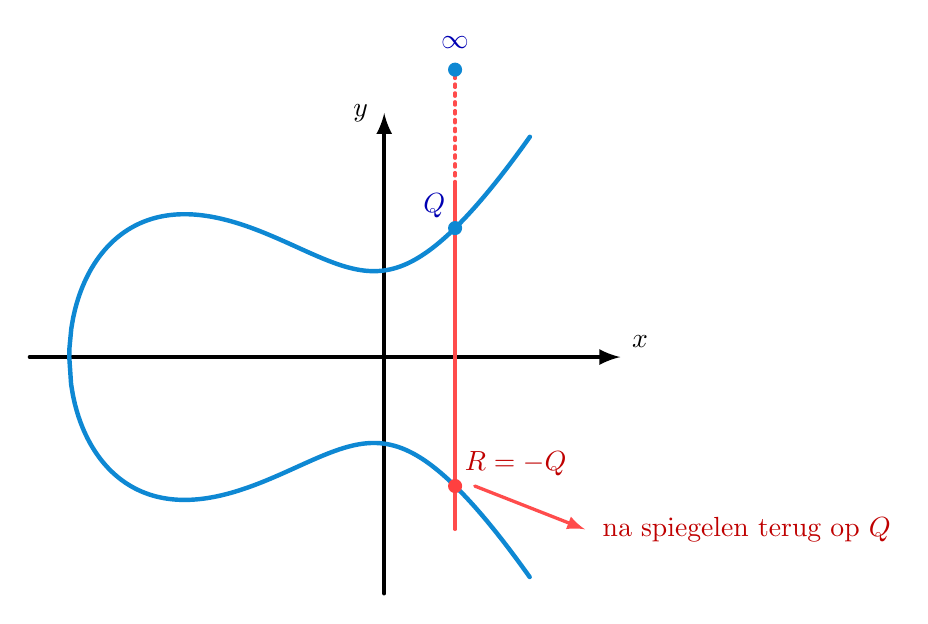
\begin{tikzpicture}[>=latex, line cap=round, line join=round]

% --- Global TikZ Styles ---
\tikzset{
    axis/.style={
        ->,
        >=latex,
        ultra thick,
        draw=black
    },
    axisline/.style={
        ultra thick,
        draw=black
    },
    elliptic/.style={
        draw=cyan!70!blue,
        line width=1.6pt
    },
    construction/.style={
        draw=red!70,
        line width=1.2pt
    },
    constructiondashed/.style={
        draw=red!70,
        dashed,
        line width=1.1pt
    },
    redpoint/.style={
        circle,
        fill=red!75,
        inner sep=1.8pt
    },
    bluepoint/.style={
        circle,
        fill=cyan!70!blue,
        inner sep=1.8pt
    }
}

% =========================================================================
% --- Neutraal element: Q + O = Q ---
% =========================================================================

% We gebruiken opnieuw de linkse kromme:
% y^2 = x^3 + 4x^2 + x + 4,
% met verticale compressie 0.55.

\pgfmathsetmacro{\k}{0.55}

% --- Axes ---
\draw[axisline] (-4.5,0) -- (2.1,0);
\draw[axis] (2.1,0) -- (3.0,0);

\draw[axisline] (0,-3.0) -- (0,0);
\draw[axis] (0,0) -- (0,3.1);

\node at (3.25,0.2) {$x$};
\node at (-0.3,3.1) {$y$};

% --- Elliptische kromme ---
\draw[elliptic]
    plot[domain=1.85:-4, samples=250]
        (\x, {\k * sqrt(abs(\x*\x*\x + 4*\x*\x + \x + 4))})
    --
    plot[domain=-4:1.85, samples=250]
        (\x, {-\k * sqrt(abs(\x*\x*\x + 4*\x*\x + \x + 4))});

% --- Punt Q en zijn inverse R = -Q ---
\pgfmathsetmacro{\xQ}{0.90}
\pgfmathsetmacro{\fQ}{\xQ*\xQ*\xQ + 4*\xQ*\xQ + \xQ + 4}
\pgfmathsetmacro{\yQ}{\k * sqrt(\fQ)}

% --- Verticale lijn door Q en O, verder naar oneindig ---
    \pgfmathsetmacro{\OheightRed}{3.65}

    \draw[construction]
        (\xQ,{-\yQ - 0.55}) -- (\xQ,{\yQ + 0.55});

    \draw[construction, dotted]
        (\xQ,{\yQ + 0.55}) -- (\xQ,\OheightRed);

    \node[bluepoint] at (\xQ,\OheightRed) {};
    \node[blue!70!black, above, yshift=4pt] at (\xQ,\OheightRed) {$\infty$};

% --- Punten op de kromme ---
\node[bluepoint] at (\xQ,\yQ) {};
\node[redpoint] at (\xQ,-\yQ) {};

% --- Labels ---
\node[blue!70!black, above left] at (\xQ,\yQ) {$Q$};
\node[red!75!black, above right] at (\xQ,-\yQ) {$R=-Q$};;

% \node[red!75!black, align=left] at (-3.9,2.45)
%     {$Q+\mathcal O=Q$};

% --- Spiegelingsaanduiding ---
\draw[construction, ->]
    ({\xQ+0.25},{-\yQ}) -- ({\xQ+1.65},{-\yQ-0.55});

\node[red!75!black, align=left, right] at ({\xQ+1.75},{-\yQ-0.55})
    {na spiegelen terug op $Q$};

\end{tikzpicture}